\newcommand*{\ls}{Locality-Sensitive}%
\newcommand*{\lsh}{Locality-Sensitive Hashing}%
\subsection{\lsh{}}\label{sub:lsh}
Πρόκειται για έναν πιθανοτικό αλγόριθμο που έχει στενή σχέση με το data clustering και το nearest neighbor search.
O αλγόριθμος \lsh{} δημιουργήθηκε με σκοπό την γρήγορη αναζήτηση σε μια μεγάλη βάση δεδομένων για την εύρεση παρόμοιων στοιχείων \cite{slaney2008locality}.
Γενικά, κάθε σημείο της βάσης τοποθετείται σε ένα \href{https://en.wikipedia.org/wiki/Hash_table}{hash bucket} σύμφωνα με μια hash function.
Συνήθως (πχ σε εφαρμογές encryption) θέλουμε μια hash function να αντιστοιχεί 2 αντικείμενα στο ίδιο hash bucket μόνο όταν είναι ίδια.
Ωστόσο, με \ls{} hash προσπαθούμε 2 αντικείμενα που είναι περίπου ίδια να τα αντιστοιχήσουμε στο ίδιο bucket.
Έτσι, κάθε νέο query ομαδοποιείται με παρόμοια αντικείμενα σε κοινό bucket.

\subsubsection{Εφαρμογή σε σύστημα QbSH}
Στη βιβλιογραφία η πρώτη αναφορά χρήσης \lsh{} σε συστήματα QbSH έγινε το \citeyear{ryynanen2008query} στο \cite{ryynanen2008query}.

\begin{wrapfigure}{r}{0.5\textwidth}
        \centering
        \vspace{-20pt}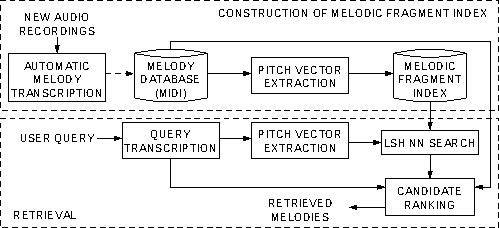
\includegraphics[width=\linewidth]{ryynanen2008query}
        \vspace{-20pt}\caption{Πρώτη χρήση LSH σε σύστημα QbSH. Block διάγραμμα από \protect\cite{ryynanen2008query}}
        \label{fig:ryynanen2008query}
\end{wrapfigure}

Η στρατηγική που ακολουθείται χωρίζεται στη
μετατροπή των queries σε μορφή που μπορεί να χρησιμοποιηθεί στην αναζήτηση και
την αντιστοίχηση των queries σε μελωδίες της βάσης.
Για κάθε pitch vector από τα queries αναζητούνται οι κοντινότεροι γείτονες από το database.
Η ομοιότητα 2 pitch vector υπολογίζεται από τη σχέση:
\begin{equation*}
\norm{p_i - p_j} = (\sum\limits_{k=1}^{d}\abs{p_i(k) - p_j(k)}^2)^{1/2}
\end{equation*}

Το block διάγραμμα της εφαρμογής φαίνεται στο \imageref{ryynanen2008query}.
Η τεχνική αυτή οδηγεί σε γρήγορες αλλά και ακριβείς αναζητήσεις.

\begin{figure}[htb]
    \centering
    \begin{subfigure}[t]{0.3\linewidth}
        \adjincludegraphics[max width=\linewidth,height=5cm, keepaspectratio]{wang2012query}
        \caption{Block διάγραμμα από \protect\cite{wang2012query}}
        \label{fig:wang2012query}
    \end{subfigure}\hfill
    \begin{subfigure}[t]{0.3\linewidth}
        \adjincludegraphics[max width=\linewidth, height=5cm, keepaspectratio]{guo2012query}
        \caption{Block διάγραμμα από \protect\cite{guo2012query}}
        \label{fig:guo2012query}
    \end{subfigure}\hfill
    \begin{subfigure}[t]{0.3\linewidth}
        \adjincludegraphics[max width=\linewidth, height=5cm, keepaspectratio]{guo2013query}
        \caption{Block διάγραμμα από \protect\cite{guo2013query}}
        \label{fig:guo2013query}
    \end{subfigure}
    \begin{subfigure}[t]{0.63\linewidth}
        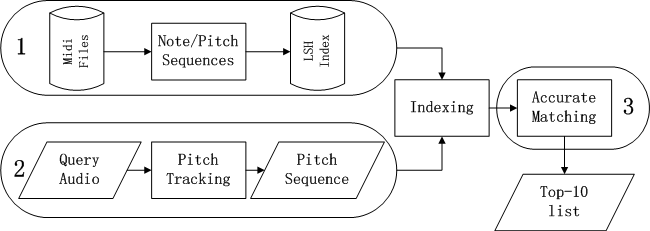
\includegraphics[width=\linewidth, keepaspectratio]{li2013mirex}
        \caption{Block διάγραμμα από \protect\cite{li2013mirex} του διαγωνισμού MIREX 2013}
        \label{fig:li2013mirex}
    \end{subfigure}
    \caption{Block διαγράμματα από συγγενικά συστήματα QbSH που χρησιμοποιούν LSH}
    \label{fig:many-lsb-blocks}
\end{figure}

Τις χρονιές 2012 και 2013 εμφανίστηκαν πιο πολύπλοκα συστήματα QbSH που χρησιμοποιούσαν \lsh{}.
Συγκεκριμένα, στο \cite{wang2012query}, του οποίου το block διάγραμμα φαίνεται στο \imageref{wang2012query},
παρουσιάζονται η μέθοδος note-based locality sensitive hashing (NLSH)
σε συνδυασμό με pitch-based locality sensitive hashing (PLSH).
%\leavevmode%
\begin{enumerate}
    \item PLSH Indexing:
    indexing με βάση τον τόνο της φωνής για γρήγορη διαγραφή των λιγότερο πιθανών υποψήφιων αποτελεσμάτων.
    \item NLSH Indexing:
    Θεωρείται δύσκολο ένα query να έχει με ακρίβεια ίδιο τόνο με το ground-truth MIDI αρχείο όταν ένας χρήστης πρέπει να κρατήσει το ύψος μιας νότα για μια συγκεκριμένη χρονική περίοδο.
    Για αυτό το λόγο αγνοείται η διάρκεια της νότας (μέχρι κάποιο επιτρεπόμενο error).
\end{enumerate}

\begin{figure}
	\centering
	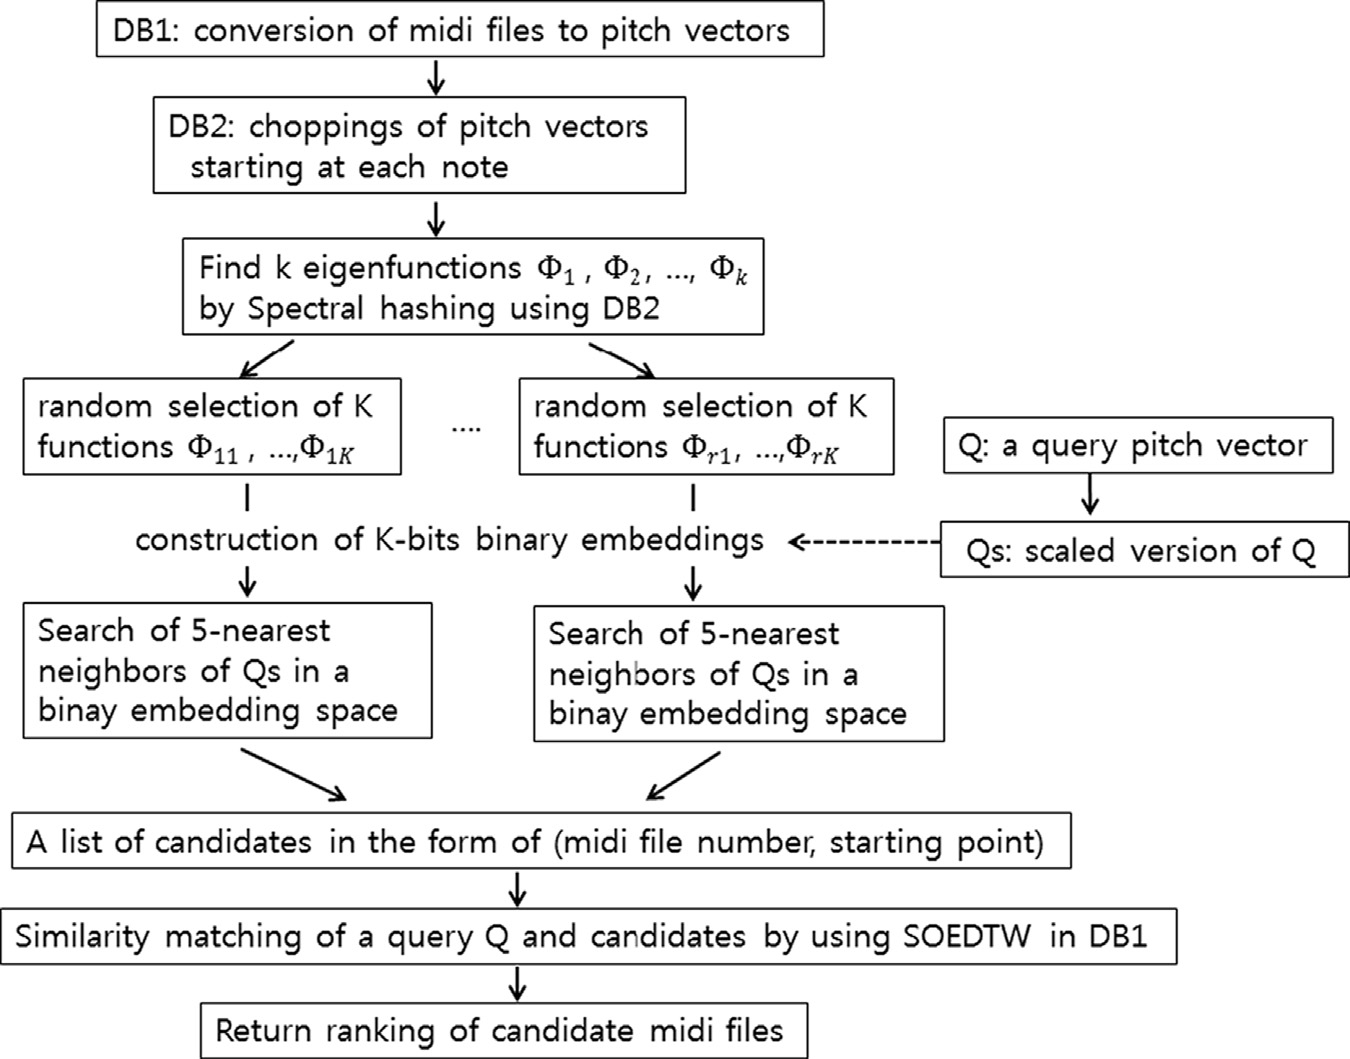
\includegraphics[width=0.8\textwidth]{park2015query}
	\caption{Block διάγραμμα από \protect\cite{park2015query} που χρησιμοποιεί multiple spectral hashing}
	\label{fig:park2015query}
\end{figure}

Τέλος, αντί για χρήση \lsh{} το \citeyear{park2015query} στο \cite{park2015query} χρησιμοποιήθηκε multiple \href{https://en.wikipedia.org/wiki/Spectral_Hash}{Spectral Hashing}.
Το block διάγραμμα φαίνεται στο \imageref{park2015query}
Το spectral hashing υλοποιείται σύμφωνα με τα \cite{weiss2009spectral,weiss2009spectral-blog} ως εξής:
%\leavevmode%
\begin{enumerate}
\item Find the principal components of the data using PCA.
\item Calculate the $k$ smallest single-dimension analytical eigenfunctions of $L_p$ using a rectangular approximation along every PCA direction.
This is done by evaluating the $k$ smallest eigenvalues for each direction, thus creating a list of $dk$ eigenvalues, and then sorting this list to find the $k$ smallest eigenvalues.
\item Threshold the analytical eigenfunctions at zero, to obtain binary code.
\end{enumerate}

\undef{\ls}
\undef{\lsh}
